\subsection{OCR}

En aquesta etapa del sistema s'ha implementat un classificador OCR (SVM) encarregat d'identificar cada caràcter individual segmentat de la matrícula (lletres i números). A partir dels blobs obtinguts en la fase de segmentació, el sistema assigna una etiqueta a cada regió mitjançant un model entrenat prèviament.

\subsubsection{Dataset Utilitzat}

Per a l'entrenament del classificador OCR s'ha utilitzat un dataset públic d'OCR disponible a Kaggle (\texttt{standard OCR dataset}), el qual conté imatges de caràcters individuals (lletres i números) organitzades en carpetes separades per classe. Cada classe conté aproximadament entre 500 i 600 imatges, proporcionant una distribució equilibrada entre caràcters.

\

El dataset s'ha carregat utilitzant un \texttt{imageDatastore} de MATLAB, configurat per llegir automàticament les subcarpetes i assignar les etiquetes segons el nom de cada carpeta. 


\subsubsection{Funcions Implementades}

Les principals funcions implementades en aquest mòdul són:

\begin{itemize}
    \item \texttt{extract\_character\_features}: funció compartida entre l'entrenament i la part de classificació. S'encarregada d'extreure el vector de característiques de cada caràcter (explicades al següent apartat).
    
    \item \texttt{classify\_character}: funció que carrega el model SVM entrenat, extreu les característiques i retorna la predicció del caràcter corresponent a una imatge d'entrada.
    
    \item \texttt{recognize\_plate}: funció que recorre tots els blobs detectats en una matrícula segmentada, aplica el classificador (classify\_character) a cada regió i construeix la cadena final de la matrícula concatenant les prediccions.
\end{itemize}

A part d'aquestes funcions principals, s'ha implementat el script que gestiona l'entrenament del model:

\begin{itemize}
    \item \texttt{train\_ocr\_classifier}: script que carrega el dataset d'OCR, divideix els conjutns de features y labels en conjunts de entrenament (80\%) i test (20\%), extreu les característiques de cada imatge amb la funció \texttt{extract\_character\_features}  i entrena un model SVM amb kernel lineal. Finalment calcula i mostra les mètriques d'avaluació (accuracy i matriu de confusió) sobre el conjunt de test.
\end{itemize}

\subsubsection{Decisions de Disseny*}

Primer de tot, respecte la selecció del dataset d'entrenament, s'han utilitzat diverses alternatives al llarg del procés. Inicialment es va utilitzar un altre datset (també d'internet) el qual contenia imatges de caràcters directament obtinguit de matrícules reals. Tot i això, es van observar diversos problemes després de fer les primeres proves. Les causes indentificades van ser que totes les imatges (de cada caracter) eren de la mateixa tipologia, per tant, el model no era capaç de generalitzar a altres fonts d'imatges de forma correcta. A més, moltes estaven rotades o deformades, i en el nostre cas això perjudicava més que ajudava ja que en el nostre pipeline es realitza una etapa d'alineació prèvia a la segmentació, per tant, els caracters sempre apareixien rectes (sense rotacions exajerades). Després de descartar aquest dataset, es va optar per utilitzar el datset d'OCR clàssic mencionat anteriorment. 

\

Per a la representació dels caràcters s'han combinat múltiples descriptors amb l'objectiu de capturar tant la forma global com les estructures internes dels símbols:

\begin{itemize}
    \item \textbf{HOG (Histogram of Oriented Gradients)}: utilitzat amb cel·les de 4x4 píxels per capturar millor els detalls fins dels caràcters, com traços i cantonades. Inicalment es van provar cel·les de 8x8, però va reduir a 4x4 degut a la mida reduïda de les imatges.
    
    \item \textbf{Densitat global}: proporció de píxels actius dins la imatge binaritzada, que ajuda a diferenciar caràcters plens de caràcters oberts. 
    
    \item \textbf{Nombre de components connectats}: mesura del nombre de components connectats de la imatge binaritzada negada, que pot ajudar a distingir caràcters amb forats (per exemple B i 8).  
    \item \textbf{Perfils de projecció}: distribució horitzontal i vertical dels píxels, normalitzada a longitud fixa, que permet capturar l'estructura general del caràcter.
    
    \item \textbf{Zoning 4x4 i 6x3}: divisió de la imatge en regions per calcular densitat local, aportant informació espacial sobre la distribució dels traços.
    
    \item \textbf{Crossing numbers}: nombre de transicions entre fons i primer pla per fila, útil per distingir caràcters amb estructures similars.
    \item etc. Por determinar
\end{itemize}

Totes les imatges es redimensionen a una mida fixa de 32x32 píxels abans de l'extracció de característiques per garantir consistència entre mostres.

\subsubsection{Alternatives Descartades*}

\subsubsection{Resultats i rendiment del classificador}

El rendiment del model s'ha avaluat utilitzant un conjunt de test independent (20\% del dataset total), amb una divisió aleatòria de les dades. La mètrica principal utilitzada ha sigut la matriu de confusió, d'on s'han tret també la mètrica de accuracy. 

\begin{figure}[H]
    \centering
    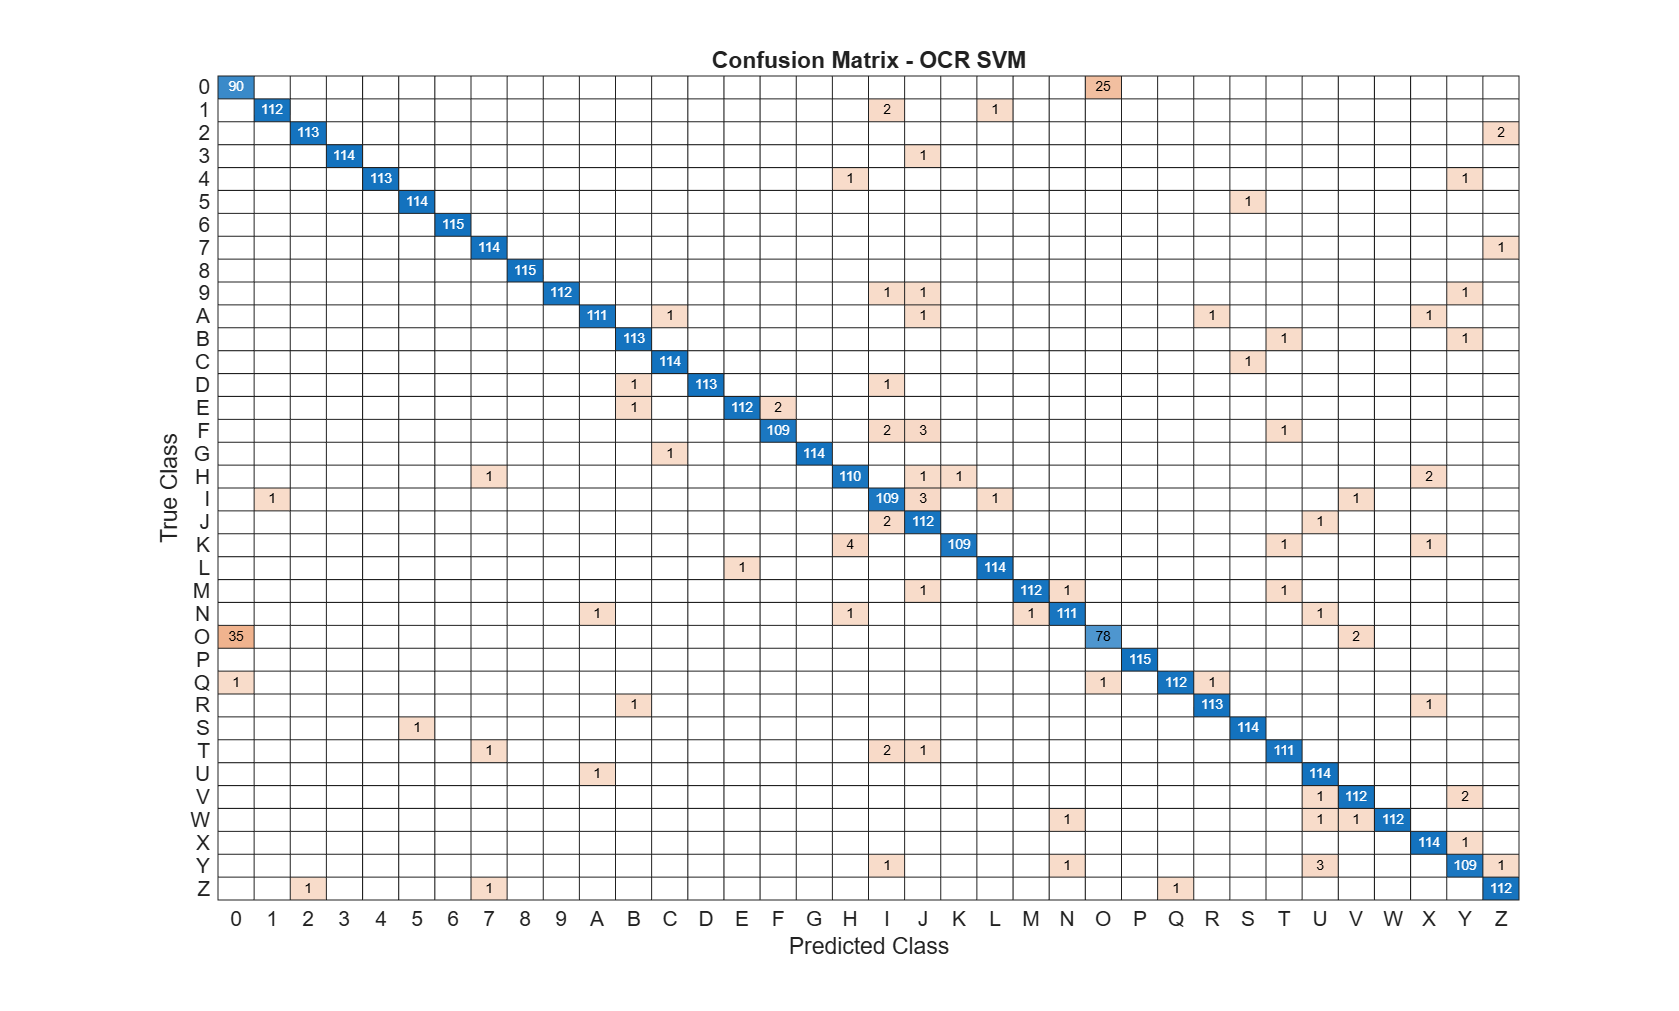
\includegraphics[width=\textwidth]{images/confusionMatrixOCR.png}
    \caption{Matriu de confusió del classificador OCR}
\end{figure}

\begin{itemize}
    \item Accuracy: 96.72\%
\end{itemize}

Com es pot observar a la matriu de confusió, el model té una bona capacitat de discriminació entre les diferents classes de caràcters, tot i que hi han casos concrets on li costa diferenciar depèn de quin caràcter. On més es pot identificar aquest problema és entre el 0 i la O, amb una quantitat considerable de confusions. Els demès errors es distribueixen de forma més dispersa i puntual. 

\subsubsection{Errors trobats*}

Tot i haver obtingut un bon rendiment amb el model de test, en les proves reals realitzades (conjuntament amb tot el pipeline) s'han detectat diversos errors de reconeixement. 

Les lletres més conflictives han sigut: 

\begin{itemize}
    \item \textbf{0 vs O}: com s'ha mencionat anteriorment, el model té dificultats per diferenciar entre el número 0 i la lletra O, especialment quan les matrícules tenen una tipografia on aquests símbols són molt similars.
    \item \textbf{W vs H}: 
\end{itemize}